\documentclass[a4paper,12pt]{book}

\usepackage[spanish, es-tabla]{babel}
\usepackage[utf8]{inputenc}


\usepackage{setspace}
\usepackage{graphicx}
\usepackage{multirow}
%\usepackage[pdftex]{graphicx}
%\usepackage{epsfig}

%\usepackage{cmbright} %Fuente tipo arial
\usepackage{mathptmx} %Fuente times roman

%\usepackage [dvips]{graphicx}

%Listados 
\usepackage{listings}%listados 
\usepackage{listingsutf8}

\renewcommand{\lstlistingname}{Listado}
\renewcommand{\chaptername}{Cap\'itulo}

   
%setup  de lstlisting
\usepackage{courier}
 \lstset{
         basicstyle=\footnotesize\ttfamily, % Standardschrift
         %numbers=left,               % Ort der Zeilennummern
         numberstyle=\tiny,          % Stil der Zeilennummern
         basicstyle=\scriptsize,		% Font size?
         %stepnumber=2,               % Abstand zwischen den Zeilennummern
         numbersep=5pt,              % Abstand der Nummern zum Text
         tabsize=1,                  % Groesse von Tabs
         extendedchars=true,         %
         breaklines=true,            % Zeilen werden Umgebrochen
%         keywordstyle=\color{red},	%Opción palabras clave en rojo
				 %keywordstyle=\color{black}\bfseries, %Opción palabras clave en negrita
				 keywordstyle=\color{black}\textbf, %Opción palabras clave en negrita
         %keywordstyle=\color{black}\bfseries\underbar, %Opción palabras clave en negrita y subrayado (\'util si no es color)
%         keywordstyle=\color{black}\bfseries\underbar,%Negrita y subrayado, problemas con algunos elementos
       frame=tb,         						%Colocal una l\'inea al final del cuadro (parte inferior)
% 				frame=single,
 %        keywordstyle=[1]\textbf,    % Stil der Keywords
 %        keywordstyle=[2]\textbf,    %
 %        keywordstyle=[3]\textbf,    %
 %        keywordstyle=[4]\textbf,   \sqrt{\sqrt{}} %
 	commentstyle=\color{gray0}\itshape,    %Color comentarios m\'as visible en grises era red
         stringstyle=\color{gray0}\ttfamily, % Farbe der String  era blue
         showspaces=false,           % Leerzeichen anzeigen ?
         showtabs=false,             % Tabs anzeigen ?
         xleftmargin=.1cm,   %era 17pt
         xrightmargin=.1cm,
         framexleftmargin=0cm,  %era17pt    %Controla la posición de la l\'inea que sirve de separador cerrando cada listado
         %framexleftmargin=1.5cm,  %era17pt    %Controla la posición de la l\'inea que sirve de separador cerrando cada listado
%         framexrightmargin=7pt,
%         framexbottommargin=4pt,
         %backgroundcolor=\color{lightgray},
         showstringspaces=false,      % Leerzeichen in Strings anzeigen ?    
        %escapeinside={}	% Para escapar a LaTeX.    
        escapeinside=@@,	% Para escapar a LaTeX y que contemple las tildes, pero no consigo que se remarque la palabra clave 
 }
 
 \lstloadlanguages{% Check Dokumentation for further languages ...
         %[Visual]Basic
         %Pascal
         %C
         %C++
         %XML
         %HTML
         %Matlab,
         Java,
         C
 }
 
\renewcommand{\contentsname}{Contenidos}

\usepackage[bookmarks,colorlinks]{hyperref}
%\usepackage{hyperref}   %Hiperenlaces dentro del documento, aconsejan como ï¿Ã�?�“ltimo


\begin{document}
 

\begin{titlepage}
\thispagestyle{empty}
\pagenumbering{gobble} 
\begin{center}
\vspace{-3.2cm}


UNIVERSIDAD DE LAS PALMAS DE GRAN CANARIA \\
Escuela de Ingenier\'ia Inform\'atica
\end{center}

\begin{center}
\vspace{1.5cm}

\includegraphics[scale=1]{Processing_Logo.png} \\
\end{center}

\begin{center}
\setstretch{1.2}
\vspace{1.5cm}
\textbf{\large Introducci\'on a la Programaci\'on con Processing}
\end{center}

\vspace{7cm}
\begin{flushleft}
	\begin{tabular}{ll}
		Modesto Castrill\'on Santana
	\end{tabular}  
\end{flushleft}  

\thispagestyle{empty}
\end{titlepage}

\setstretch{1}

\setcounter{tocdepth}{4}
\setcounter{secnumdepth}{4}

\tableofcontents%

\newpage
\pagenumbering{arabic}
\setcounter{page}{1}

\chapter{Introducci\'on a Processing}

\section{Introducci\'on}

\textbf{Processing} es un proyecto de c\'odigo abierto con fines creativos que se basa en el lenguaje Java, se concibe como un cuaderno de dibujo 
para artistas inform\'aticos, programadores y dise\~nadores, siendo muy utilizado en dichas comunidades por su facilidad de uso. 
La facilidad sint\'actica de Java, 
y la enorme comunidad existente, sirven de gran apoyo, ofreciendo un conjunto de herramientas de c\'odigo abierto para la creaci\'on de aplicaciones creativas. Su dise\~no pretende facilitar la programaci\'on que integre im\'agenes, animaci\'on, sonido e interacci\'on. 


Es utilizado por estudiantes, artistas, dise\~nadores, investigadores y aficionados tanto para el aprendizaje, como la creaci\'on de
prototipos y la producci\'on audiovisual. De esta forma cubre necesidades no s\'olo para ense\~nar los fundamentos de programaci\'on, sino tambi\'en como cuaderno de prototipos software, o herramienta de producci\'on profesional. 
Processing est\'a disponible en el siguiente enlace \href{http://processing.org/}{Processing\footnote{http://processing.org/}}, si bien
en la secci\'on de referencias se relacionan otros recursos con ejemplos y demos.

\section{Instalaci\'on y entorno de programaci\'on}

La instalaci\'on requiere realizar la descarga a trav\'es de processing.org, y descomprimir. Una vez realizados los preparativos, tras lanzar el entorno se te presenta la interfaz, si no hubieras
activado la interfaz en espa\~nol, y quisieras cambiarla, prueba a  a trav\'es del men\'u 
con \textit{File $\rightarrow$ Preferences}. No olvides que es posible acceder a los ejemplos
a trav\'es de la barra de men\'u \textit{Archivo $\rightarrow$ Ejemplos}.


El entorno de desarrollo de Processing (PDE), ver figura~\ref{fig:processing_entorno}, consiste en un simple editor de texto para escribir c\'odigo, un \'area de mensajes, una consola
de texto, fichas de gesti\'on de archivos, una barra de herramientas con botones para las acciones comunes, y una serie de men\'us. Cuando
los programas se ejecutan, se abren en una nueva ventana llamada la ventana de visualizaci\'on (\textit{display window}).

\begin{figure}[ht]
  \centering
  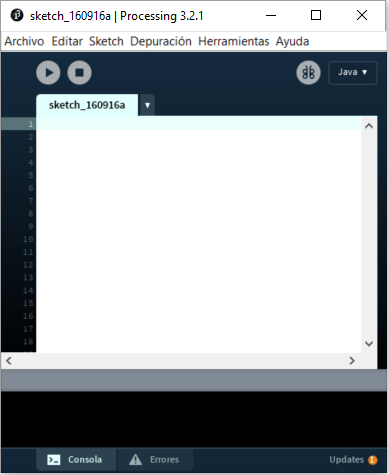
\includegraphics[width=0.7\linewidth]{processing-entorno.png}
  \caption{Imagen del entorno de programaci\'on, PDE, de Processing.}
  \label{fig:processing_entorno}
\end{figure}

Cada pieza de software escrito con Processing se denomina boceto o \textit{sketch}. Se escribe a trav\'es del editor de texto, disponiendo de las funciones t\'ipicas
para cortar y pegar, as\'i como las de b\'usqueda y reemplazo de texto. 

El \'area de mensajes, en la parte inferior, ofrece informaci\'on de la salida de texto del programa en ejecuci\'on,
al hacer uso de las funciones \textit{print()} y \textit{println()},
adem\'as de mensajes de error, tanto en ejecuci\'on como durante la edici\'on. Las utilidades para la 
depuraci\'on integradas en el entorno est\'an disponibles desde la versi\'on 2.0b7.

Los botones de la barra de herramientas permiten ejecutar y detener programas, 
ver Tabla~\ref{tab:comandos}.
 Comandos adicionales se encuentran dentro de la barra de men\'u: \textit{Archivo}, \textit{Editar}, \textit{Sketch}, \textit{Depuraci\'on}, \textit{Herramientas},
 \textit{Ayuda}. Los submen\'us son sensibles al contexto,  lo que significa que 
 s\'olo los elementos pertinentes a la labor que se est\'a llevando a cabo est\'an disponibles. 

\begin{table}[ht]
\caption{Resumen de comandos habituales}
\centering
\begin{tabular}{|c|c|l|}
\hline
\multirow{2}{*}{
\includegraphics[scale=0.68]{processing_ejecutar.png}}&\multirow{2}{*}{Ejecutar} & Compila el c\'odigo, abre una ventana de visualizaci\'on,\\
& & y ejecuta el programa\\ \hline
\multirow{2}{*}{
\includegraphics[scale=0.7]{processing_detener.png}}&\multirow{2}{*}{Detener} & Finaliza la ejecuci\'on de un programa\\
& & \\\hline
% \multirow{2}{*}{
\includegraphics[scale=0.75]{processing_nuevo.png}}&\multirow{2}{*}{Nuevo} & Crea un nuevo sketch o proyecto en la ventana actual\\
% & & Utilice \textit{Archivo $\rightarrow$ Nuevo}
% 
% para crearlo en una nueva ventana\\\hline
% \multirow{2}{*}{
\includegraphics[scale=0.7]{processing_abrir.png}}&\multirow{2}{*}{Abrir} & Abre un archivo en la ventana actual. Utilice \\
% & & \textit{Archivo $\rightarrow$ Abrir} para crearlo en una nueva ventana\\ \hline
% \multirow{2}{*}{
\includegraphics[scale=0.7]{processing_guardar.png}}&\multirow{2}{*}{Guardar} & Guarda el proyecto actual \\
% & & \\\hline
% \multirow{2}{*}{
\includegraphics[scale=0.75]{processing_exportar.png}}&\multirow{2}{*}{Exportar} & Exporta el proyecto actual como un applet de Java embebido \\
% & & en un archivo HTML \\\hline
\end{tabular}
\label{tab:comandos}
\end{table}




\section{Programaci\'on en modo b\'asico}

Processing permite varios modos de programaci\'on: el modo b\'asico, y el modo continuo. Mencionaremos brevemente ambos, para concluir con los \textit{applets}. 

El modo b\'asico permite la elaboraci\'on de im\'agenes est\'aticas, es decir que no se modifican, adem\'as de poder ser \'util para aprender los fundamentos de la programaci\'on. 
L\'ineas simples de c\'odigo tienen una representaci\'on directa en la pantalla. 


\subsection{Dibujo de primitivas b\'asicas}

Un ejemplo m\'inimo de dibujo de una l\'inea entre dos puntos de la pantalla.

\begin{lstlisting}[frame=single,caption={Ejemplo de dibujo de una l\'inea},label=code:processing-linea]
line(0,0,10,10);
\end{lstlisting}

Se debe tener en cuenta que se emplea el sistema de coordenadas cartesiano, como es habitual, teniendo su origen en la esquina superior izquierda como 
se muestra en las figuras~\ref{fig:coordenadas} y~\ref{fig:processing_ejes}.
Si se define  una ventana de $320 \times 240$
p\'ixeles, la coordenada $[0, 0]$ se corresponde con la esquina superior izquierda como se ilustra en la 
figura~\ref{fig:coordenadas}.

\begin{figure}[h]
  \centering
  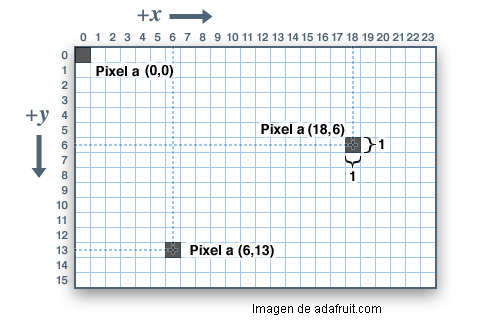
\includegraphics[width=0.7\linewidth]{Scoordenadas.png}
  \caption{Sistema de coordenadas de la pantalla.}
  \label{fig:coordenadas}
\end{figure}


\begin{figure}[h]
  \centering
  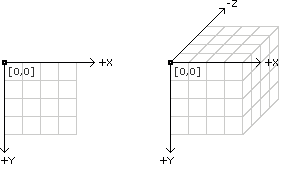
\includegraphics[scale=0.7]{processing_ejes.png}
  \caption{Sistema de coordenadas en 2 y 3 dimensiones.}
  \label{fig:processing_ejes}
\end{figure}



Processing tambi\'en puede simular el dibujo en tres dimensiones. En la superficie de la imagen, 
la coordenada \textit{z} es cero, con valores 
\textit{z} negativos movi\'endose hacia atr\'as en el espacio. Cuando se realiza el dibujo en 3D simulado, la c\'amara se coloca en el centro de la pantalla.




Un siguiente paso lo damos al dibujar dos l\'ineas modificando el color del pincel con la funci\'on \textit{stroke}. En este \href{http://www.w3schools.com/colors/colors_rgb.asp}{enlace} puedes practicar con el espacio de color RGB
(rojo, verde y azul) modificando los valores de cada canal.
RGB es el modelo de color por defecto que puede  modificarse con \textit{colormode()}.

\begin{lstlisting}[frame=single,caption={Dibujo de dos l\'ineas modificando el color},label=code:processing-lineascolor]
stroke(255,0,0);//Tripleta RGB
line(0,0,10,10);

stroke(0,255,0);
line(30,10,10,30);
\end{lstlisting}

Indicar que con el comando \textit{stroke}, puede especificarse un \'unico valor, entre 0 y 255, que se interpreta como tono de gris, p.e. \textit{stroke(0);} especifica el color negro, y \textit{stroke(255);} el blanco. Es tambi\'en posible indicar la tripla RGB como un valor hexadecimal \textit{stroke(\#9ACD32)};.

Tambi\'en es posible establecer de forma arbitraria el tama\~no de la ventana de visualizaci\'on con el comando \textit{size()}.


\begin{lstlisting}[frame=single,caption={Una l\'inea en una ventana mayor},label=code:processing-ventana]
size(640, 360); 
stroke(255,0,0);
line(0,0,10,10);
\end{lstlisting}

Si no nos decidimos con el color, o simplemente queremos que cambie con cada ejecuci\'on, podemos escogerlo aleatorio haciendo uso de \textit{random()}.

\begin{lstlisting}[frame=single,caption={Dibujo de una l\'inea con color aleatorio},label=code:processing-lineacoloraleatorio]
size(640, 360); 
stroke(random(255),random(255),random(255));
line(0,0,10,10);
\end{lstlisting}

Una vez que comprendemos el dibujo de l\'ineas, para pintar un cuadrado podemos hacer uso de cuatro l\'ineas bien colocadas.
Sugiero deducir las coordenadas de los cuatro v\'ertices antes en papel.

\begin{lstlisting}[frame=single,caption={Dibujo de un cuadrado con cuatro l\'ineas},label=code:processing-cuadrado4lineas]
background(128);

size(400,400);

strokeWeight(2); //Modifica el grosor del pincel
line(30,30,30,60);
line(30,60,60,60);
line(60,60,60,30);
line(60,30,30,30);
\end{lstlisting}

Realmente existen comandos que facilitan el dibujo de otras primitivas sencillas. Para conocer todas las primitivas 2D, ver 2D primitives en \textit{Ayuda $\rightarrow$ Referencia}.

\begin{lstlisting}[frame=single,caption={Dibujo de un cuadrado},label=code:processing-rect]
stroke(255,255,255);
rect(0,0,10,10);
\end{lstlisting}

El color de relleno se define con \textit{fill()}, afectando a las primitivas a partir de ese momento. Las funciones \textit{noFill} 
y \textit{noStroke}
cancelan respectivamente el relleno y el borde de las primitivas.

\begin{lstlisting}[frame=single,caption={Dibujo de una cuadrado s\'olido},label=code:processing-fill]
stroke(255,0,255);
fill(232,123,87);
rect(0,0,10,10);
\end{lstlisting}

En todos los comandos que define un color, la especificaci\'on de un \'unico valor se interpreta como nivel de gris 
(0 negro, 255 blanco). Si se indicaran 4, el \'ultimo define la transparencia, el canal alfa.

A modo de resumen, el siguiente c\'odigo muestra el uso de varias primitivas 2D.

\begin{lstlisting}[frame=single,caption={Primitivas 2D},label=code:dibujando]
size(450,450);

stroke(128);
fill(128);

ellipse(200,300,120,120); //Por defecto modo con coordenadas del centroy di\'ametro

stroke(255,0,255);
noFill();
strokeWeight(2);
ellipse(400,300,60,60);  

stroke(123, 0, 255);
strokeWeight(10);
ellipse(40,123,60,60);  

stroke(0);
strokeWeight(1);
line(40,123,400,300);

triangle(10, 240, 50, 245, 24, 280);

fill(0);
rect(190,290,30,50);

stroke(255,0,0);
fill(255,0,0);
bezier(5,5,10,10,310,320,320,20);
\end{lstlisting}

\textbf{Te propongo componer un dibujo combinando varias primitivas y colores (\textit{rect}, \textit{ellipse}, \textit{line}, ...), ver por ejemplo el Mondrian de la figura~\ref{fig:mondrian}.}

\begin{figure}[h]
  \centering
  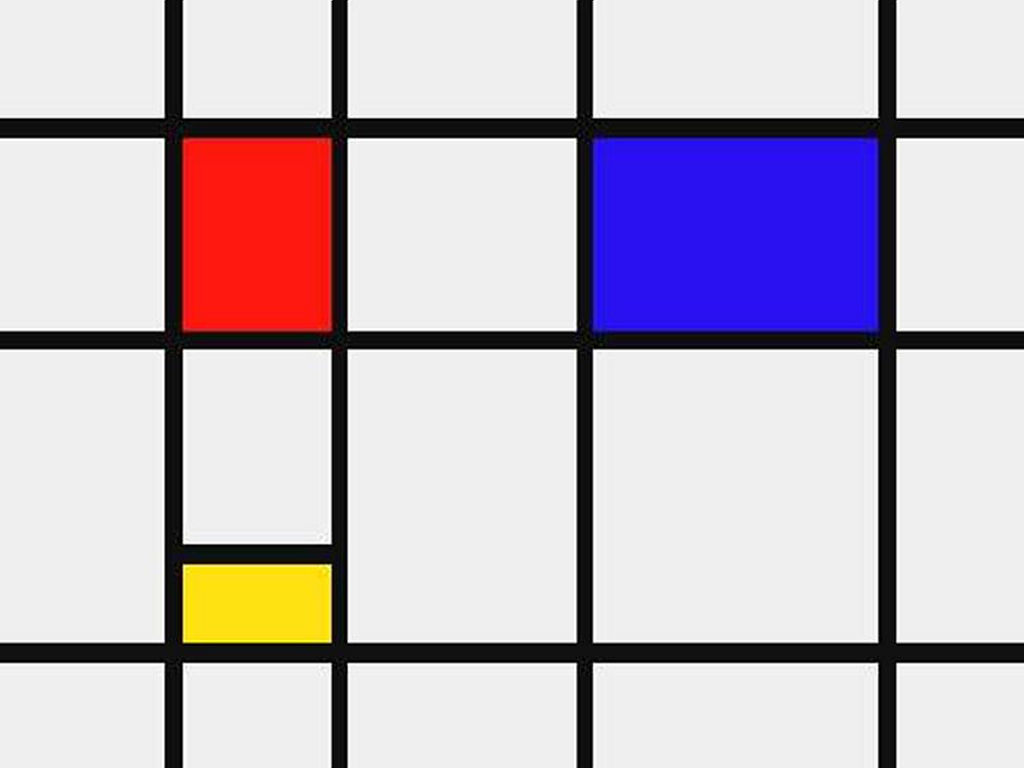
\includegraphics[width=0.4\linewidth]{mondrian.jpg}
  \caption{Piet Mondrian, \textit{Composici\'on con rojo, amarillo y azul} (1930).}
  \label{fig:mondrian}
\end{figure}

\subsection{Variables}

Un paso m\'as supone el uso de variables en el c\'odigo. Para comenzar, ilustramos en uso de variables con aquellas presentes durante la ejecuci\'on, 
como son las dimensiones de la ventana que se almacenan respectivamente en las variables \textit{width} y \textit{height}, y que utilizamos en el siguiente c\'odigo para pintar una estrella simple en el centro de la ventana, independientemente de las dimensiones que le fijemos con \textit{size()}.

\begin{lstlisting}[frame=single,caption={Dibujo de una estrella o asterisco},label=code:processing-estrella]
line(width/2-10,height/2-10,width/2+10,height/2+10);
line(width/2+10,height/2-10,width/2-10,height/2+10);
line(width/2,height/2-10,width/2,height/2+10);
line(width/2+10,height/2,width/2-10,height/2);
\end{lstlisting}

Cada variable es b\'asicamente un alias o s\'imbolo que nos permite hacer uso de una zona de almacenamiento en memoria. 
Dado que recordar la direcci\'on de memoria, un valor num\'erico, es engorroso, se hace uso de un nombre o 
identificador que permite darle mayor sem\'antica a aquello que contiene la variable. En el caso de las 
variables del sistema mencionadas, \textit{width} es una variable que justamente almacena el ancho de la ventana.
Las variables se caracterizan por el nombre, el valor que contienen, su direcci\'on, y el tipo de datos.

\textbf{Modifica el ejemplo para pintar una estrella de mayor radio, es decir mayor que 10.}

Una gran ventaja del uso de variables es que un programador puede definir y utilizar sus propias variables a conveniencia. 
Para ello en Processing es necesario declarar cualquier variable antes de utilizarla. El siguiente ejemplo utiliza 
\textbf{l} para establecer el tama\~no de la estrella.

\begin{lstlisting}[frame=single,caption={Dibujo de una estrella variable},label=code:processing-estrellavar]
int l=10;

line(width/2-l,height/2-l,width/2+l,height/2+l);
line(width/2+l,height/2-l,width/2-l,height/2+l);
line(width/2,height/2-l,width/2,height/2+l);
line(width/2+l,height/2,width/2-10,height/2);
\end{lstlisting}

En este nuevo ejemplo pintamos una l\'inea y un c\'irculo de un determinado radio, haciendo uso de la funci\'on \textit{ellipse} definiendo 
previamente el color de relleno.

\begin{lstlisting}[frame=single,caption={Dibujo de un c\'irculo },label=code:processing-ellipse]
int Radio = 50 ;

size(500,500);
background(0);
stroke(80);
line(230,220,285,275);
fill(150,0,0);
ellipse(210,100,Radio,Radio);
\end{lstlisting}


\subsection{Repeticiones}

Pensemos en crear una ventana de dimensiones $800 \times 800$ en la que pintamos l\'ineas 
verticales de arriba a abajo cada $100$ p\'ixeles. recordar que la coordenada \textit{y} de a parte
superior es $0$, y la inferior es $800$ o \textbf{height} si usamos la variable correspondiente.

\begin{lstlisting}[frame=single,caption={Dibujo de varias l\'ineas verticales},label=code:processing-lineasverticales]
size(800,800);
background(0);
stroke(255);
line(100,1,100,height);
line(200,1,200,height);
line(300,1,300,height);
line(400,1,400,height);
line(500,1,500,height);
line(600,1,600,height);
line(700,1,700,height);
\end{lstlisting}


Realmente las llamadas a la funci\'on \textit{line} son todas muy similares, s\'olo var\'ian las coordenadas \textit{x} de los 
dos puntos. Los lenguajes de programaci\'on facilitan la especificaci\'on de llamadas repetidas por medio del uso de 
bucles. Una versi\'on m\'as compacta del dibujo de las l\'ineas verticales. El bucle define una variable, \textbf{i}, a la 
que asignamos
un valor inicial $100$, un valor final, $700$, y la forma en que se va modificando \textbf{i} con cada 
ejecuci\'on, en este caso a\~nadiendo $100$.

\begin{lstlisting}[frame=single,caption={Dibujo de varias l\'ineas verticales},label=code:processing-lineasverticales2]
size(800,800);
background(0);
stroke(255);
for (int i=100;i<=700;i=i+100){
line(i,1,i,height);
}\end{lstlisting}

Particularmente \'util cuando las repeticiones son cientos o miles. 
?`C\'omo lo modificar\'ias para hacer adem\'as l\'ineas horizontales?

\subsection{Dibujar un tablero de ajedrez} 

Como tarea similar podemos plantear el dibujo de un tablero de ajedrez, que contiene $64$ casillas como 
muestra la figura~\ref{fig:tablero}. 
Fijando el fondo a blanco, los cuatro recuadros de la primera fila del tablero de ajedrez.


\begin{figure}[h]
  \centering
  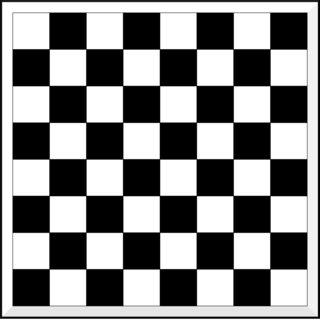
\includegraphics[width=0.35\linewidth]{chessboard.jpeg}
  \caption{Rejilla estilo tablero de ajedrez.}
  \label{fig:tablero}
\end{figure}





\begin{lstlisting}[frame=single,caption={Dibujo de una rejilla},label=code:processing-chess1]
size(800,800);
background(255);
fill(0);
//Primera fila
rect(0,0,100,100);
rect(200,0,100,100);
rect(400,0,100,100);
rect(600,0,100,100);
\end{lstlisting}

Haciendo uso de un bucle \textit{for} para pintar esas cuatro casilas negras

\begin{lstlisting}[frame=single,caption={Dibujo de una rejilla con un bucle},label=code:processing-chess2]
size(800,800);
background(255);
fill(0);
//Primera fila

for (int i=0;i<=600;i=i+200){
  rect(i,0,100,100);
}
\end{lstlisting}

Pintamos cuatro filas, cada una con su bucle particular.

\begin{lstlisting}[frame=single,caption={Dibujo de una rejilla con varios bucles},label=code:processing-chess3]
size(800,800);
background(255);
fill(0);
//Primera fila

for (int i=0;i<=600;i=i+200){
  rect(i,0,100,100);
}
for (int i=0;i<=600;i=i+200){
  rect(i,200,100,100);
}
for (int i=0;i<=600;i=i+200){
  rect(i,400,100,100);
}
for (int i=0;i<=600;i=i+200){
  rect(i,600,100,100);
}
\end{lstlisting}

Realmente cada bucle es similar a los dem\'as, sabiendo que es posible anidar bucles, con un bucle doble queda mucho m\'as 
compacto.

\begin{lstlisting}[frame=single,caption={Dibujo de una rejilla de ajedrez},label=code:processing-chess4]
size(800,800);
background(255);
fill(0);
//Primera fila

for (int j=0;j<=600;j=j+200){
  for (int i=0;i<=600;i=i+200){
    rect(i,j,100,100);
  }
}
\end{lstlisting}

Nos quedan las otras cuatro filas, que resultan de una leve variaci\'on ya que se alternan los tonos blancos y negros.

\begin{lstlisting}[frame=single,caption={Dibujo de un tablero de ajedrez},label=code:processing-chess5]
size(800,800);
background(255);
fill(0);
//Primera fila

for (int j=0;j<=600;j=j+200){
  for (int i=0;i<=600;i=i+200){
    rect(i,j,100,100);
    rect(i+100,j+100,100,100);
  }
}
\end{lstlisting}


El modo b\'asico permite componer una imagen, es el caso de los ejemplos previos, y del que se muestra a continuaci\'on. 
Es posible modificar los argumentos de las llamadas, eliminar 
comandos, o a\~nadir otros, pero el resultado es siempre est\'atico, no hay movimiento.

\begin{lstlisting}[frame=single,caption={Modo b\'asico},label=code:processing-basico]
int Radio = 50;
void setup()
{
  size(500,500);
  background(0);
  stroke(80);
  line(230, 220, 285, 275);
  fill(150,0,0);
  ellipse(210, 100, Radio, Radio);
}
\end{lstlisting}




%%%%%%%%%%%%%%%%%%%%%%%%%%%%%%%




\section{Programaci\'on en modo continuo}

\subsection{El bucle infinito de ejecuci\'on}


El modo continuo, cuenta con dos m\'etodos b\'asicos: 
 
\begin{itemize}
\item \textit{setup()} que se ejecuta una vez cuando comience el programa
\item \textit{draw()} que por defecto se ejecuta de forma continua. Este m\'etodo permite la escritura de 
funciones personalizadas, y hacer uso de la interacci\'on.
\end{itemize}

El siguiente ejemplo usa ambos m\'etodos, delimitando con llaves las instrucciones asociadas a cada uno de ellos. En concreto
 el m\'etodo \textit{setup} realiza la inicializaci\'on, en este caso fija las dimensiones de la ventana,
siendo el m\'etodo \textit{draw} el encargado de dibujar. En este caso concreto el m\'etodo \textit{draw} pinta una l\'inea con color
y posici\'on aleatoria. La gran diferencia del modo continuo es que las instrucciones contenidas en el m\'etodo \textit{draw} no se
ejecutan una sola vez, sino que se \textit{llama} a dicho m\'etodo de forma reiterada cada segundo, por defecto $40$, el resultado 
lo ver\'as al probarlo.

\begin{lstlisting}[frame=single,caption={Ejemplo de dibujo de l\'ineas de colores y posici\'on aleatoria},label=code:processing-lineasrandom]
void setup()
{
  size(400, 400);
}

void draw()
{
  stroke(random(255),random(255),random(255));	
  line(random(width),random(height),random(width),random(height));
}
\end{lstlisting}


Si s\'olo hacemos uso del m\'etodo \textit{setup}, el resultado es equivalente al modo b\'asico, dado 
que dicho m\'etodo se ejecuta una \'unica vez.

\begin{lstlisting}[frame=single,caption={Ejemplo b\'asico},label=code:processing-primer]
void setup()
{
  size (240,240); 		// Dimensiones del lienzo
  background(128,128,128); 	// Color de lienzo en formato RGB
  noStroke(); 			// Sin borde para las figuras
  fill(0); 			// Color de relleno de las figuras (0 es negro)
  rect(100, 100, 30, 30); 	// Esquina superior izquierda, ancho y alto
}
\end{lstlisting}

  
El siguiente ejemplo dibuja cuatro c\'irculos en la pantalla y utiliza adem\'as una funci\'on propia llamada \textit{circles()}. 
Observa el modo en que se define, y el uso de las llaves para delimitar las instrucciones contenidas en la funci\'on.
En este caso concreto, el c\'odigo de 
\textit{draw()} s\'olo se 
ejecuta una vez, porque en \textit{setup()} se llama a la funci\'on \textit{noLoop()}, que cancela la repetici\'on, resultando 
equivalente al modo b\'asico.
 

 \begin{lstlisting}[frame=single,caption={Ejemplo de uso del m\'etodo \textit{draw}},label=code:processing-circlesc]
void setup() {
  size(200, 200);
  noStroke();
  background(255);
  fill(0, 102, 153, 204);
  smooth();
  noLoop();
}

void draw() {
  circles(40, 80);
  circles(90, 70);
}

void circles(int x, int y) {
  ellipse(x, y, 50, 50);
  ellipse(x+20, y+20, 60, 60);
}
 \end{lstlisting}

En general la ejecuci\'on reiterada tiene sentido cuando exista un cambio en aquello que dibujamos ya sea por movimiento, modificaci\'on
del color, etc. Veamos un ejemplo de dibujado de l\'ineas desde un punto fijo, con el otro extremo aleatorio, 
variando tambi\'en el color de forma aleatoria.

\begin{lstlisting}[frame=single,caption={Dibujo de l\'ineas desde un punto},label=code:processing-lineasdesdepunto]
void setup() {
  size(400, 400); 
  background(0);
}

void draw() { 
  stroke(0,random(255),0);  
  line(50, 50, random(400), random(400));
}
\end{lstlisting}

En esta ocasi\'on forzamos a que sean l\'ineas aleatorias, pero verticales y blancas.

\begin{lstlisting}[frame=single,caption={Dibujo de l\'ineas blancas verticales},label=code:processing-lineasv]
void setup() {
  size(400, 400); 
}

void draw() { 
  stroke(255);
  
  float dist_izq=random(400); 
  line(dist_izq, 0, dist_izq, 399);
}

Variando el color

void setup() {
  size(400, 400); 
}

void draw() { 
  stroke(random(200,256),random(200,256),random(50,100));//entre dos valores
  
  float dist_izq=random(400); 
  line(dist_izq, 0, dist_izq, 399);
}
\end{lstlisting}

El color de fondo de la ventana se fija con la llamada al m\'etodo \textit{background}.

\begin{lstlisting}[frame=single,caption={Modificando el color de fondo},label=code:processing-fondo]
La tasa de refresco

void setup() {
  size(400, 400); 
	frameRate(4);
}

void draw() { 
 background(random(255));  
}
\end{lstlisting}

Nos puede ser \'util si queremos forzar que se borre la pantalla antes de dibujar de nuevo.


\begin{lstlisting}[frame=single,caption={Ejemplo de dibujo con borrado},label=code:processing-borrado]
void setup()
{
  size(400, 400);
}

void draw()
{
  background(51);  //Borra cada vez antes de pintar
  stroke(random(255),random(255),random(255));
  line(random(width),random(height),random(width),random(height));
}
\end{lstlisting}

El siguiente ejemplo introduce el uso del m\'etodo \textit{frameRate}, que fija el n\'umero de llamadas al
m\'etodo \textit{draw} por segundo. En este
caso dibuja l\'ineas aleatorias, pero observa la tasa de refresco.


\begin{lstlisting}[frame=single,caption={Ejemplo de dibujo de l\'ineas a distinta frecuencia},label=code:processing-lineash]
void setup() {
  size(400, 400); 
  frameRate(4);
}

void draw() { 
  background(51);
 
  line(0, random(height), 90, random(height));
}
\end{lstlisting}


La tasa de refresco se controla a trav\'es de una serie de funciones, adem\'as de con \textit{frameRate()}:

\begin{itemize}
\item \textit{loop()}: Reestablece las llamadas a \textit{draw()}, es decir el modo continuo.
\item \textit{noLoop()}: Detiene el modo continuo, no se realizan llamadas a \textit{draw()}.
\item \textit{redraw()}: Llama a \textit{draw()} una s\'ola vez.
\end{itemize}

El siguiente c\'odigo var\'ia la tasa de refresco en base al n\'umero de ejecuciones y el evento de pulsado de
un bot\'on del rat\'on.

\begin{lstlisting}[frame=single,caption={Controlando la tasa de refresco},label=code:processing-framerate]
 
int frame = 0;
void setup() {
  size(100, 100);
  frameRate(30);
}
void draw() 
{
  if (frame > 60) 
  {  // Si han pasado 60 ejecuciones (frames) desde el comienzo
		noLoop();    	// para el programa
		background(0);   // y lo pone todo a negro.
  } 
  else 
  {       	// En otro caso, pone el fondo
		background(204); // a un gris claro 
		line(mouseX, 0, mouseX, 100); // dibuja
		line(0, mouseY, 100, mouseY);
		frame++;
  }
}
void mousePressed() {
  loop();
  frame = 0;
}
\end{lstlisting}

Un ejemplo de llamada a \textit{redraw}.

\begin{lstlisting}[frame=single,caption={Ejemplo con redraw},label=code:processing-redraw]
void setup() 
{
  size(100, 100);
}
void draw() {
  background(204);
  line(mouseX, 0, mouseX, 100);
}
void mousePressed() {
  redraw(); // Llama a draw() una vez
}
\end{lstlisting}


Por defecto se establece el modo continuo con una frecuencia de $40$ llamadas por segundo al m\'etodo \textit{draw()}, 
el siguiente c\'odigo provoca el desplazamiento 
de un c\'irculo por la ventana.
 
\begin{lstlisting}[frame=single,caption={Desplazamiento del c\'irculo},label=code:processing-loop]
int Radio = 50;
int cuenta = 0;

void setup()
{
  size(500,500);
  background(0);
}

void draw()
{
  background(0);
  stroke(175,90);
  fill(175,40);
  println("Iteraciones: " + cuenta);
  ellipse(20+cuenta, height/2, Radio, Radio);
  cuenta++;
}
\end{lstlisting}


No olvidemos que adem\'as de dibujar, es posible escribir.

\begin{lstlisting}[frame=single,caption={Hola mundo},label=code:processing-holamundo]
void setup()
{
  background(128,128,128); // Color de lienzo en formato RGB
  noStroke(); 				// Sin borde para las figuras
  fill(0); 						// Color de relleno de las figuras (0 es negro)

  // Carga una fuente en particular
  textFont(createFont("Georgia",24));
  textAlign(CENTER, CENTER);

  // Escribe en la ventana
  text("'!Hola mundo!", 100,100);
}
\end{lstlisting}

\subsection{Im\'agenes}

La funci\'on \textit{loadImage} facilita la carga de im\'agenes desde disco, que puede ser visualizada con \textit{image}.


\begin{lstlisting}[frame=single,caption={Carga de imagen},label=code:processing-imagen]
PImage img;

void setup(){
  size(600,400);
  
  img=loadImage("C:\\Users\\Modesto\\Documents\\basu.png");
}

void draw(){
  image(img,0,0);
}
\end{lstlisting}

Jugando con un desplazamiento aleatorio en la visualizaci\'on de la imagen provocamos un efecto de tembleque.

\begin{lstlisting}[frame=single,caption={Imagen que tiembla},label=code:processing-imagentiembla]
PImage img;

void setup(){
  size(600,400);
  
  img=loadImage("C:\\Users\\Modesto\\Documents\\basu.png");
}

void draw(){
  image(img,random(10),random(10));
}
\end{lstlisting}

La funci\'on \textit{tint} permite variar la intensidad de la visualziaci\'on.


\begin{lstlisting}[frame=single,caption={Variando la intensidad de la imagen},label=code:processing-intensidadimagen]
PImage img;

void setup(){
  size(600,400);
  
  img=loadImage("C:\\Users\\Modesto\\Documents\\basu.png");
}

void draw(){
  tint(mouseX/2);
  image(img,random(10),random(10));
}
\end{lstlisting}

Cargando varias im\'agenes de un ciclo, podemos almacenarlas en una lista o vecor, y mostrarla de forma consecutiva, consiguiendo el efecto de animaci\'on.


\begin{lstlisting}[frame=single,caption={Ciclo de animaci\'on},label=code:processing-cicloanima]
PImage [] img=new PImage [6];
int frame=0;

void setup(){
  size(600,400);
  
  img[0]=loadImage("C:\\Users\\Modesto\\Dropbox\\ExpertoVideoJuegos\\Ciclo1.png");
  img[1]=loadImage("C:\\Users\\Modesto\\Dropbox\\ExpertoVideoJuegos\\Ciclo2.png");
  img[2]=loadImage("C:\\Users\\Modesto\\Dropbox\\ExpertoVideoJuegos\\Ciclo3.png");
  img[3]=loadImage("C:\\Users\\Modesto\\Dropbox\\ExpertoVideoJuegos\\Ciclo4.png");
  img[4]=loadImage("C:\\Users\\Modesto\\Dropbox\\ExpertoVideoJuegos\\Ciclo5.png");
  img[5]=loadImage("C:\\Users\\Modesto\\Dropbox\\ExpertoVideoJuegos\\Ciclo6.png");
  
  frameRate(6);
}

void draw(){
  background(128);
  image(img[frame],0,0);
  
  frame=frame+1;
  if (frame==6){
    frame=0;
  }
}
\end{lstlisting}



\subsection{Control}

En un ejemplo previo desplaz\'abamos un c\'irculo por la ventana haciendo uso de una variable. Recuperamos
el desplazamiento en 
horizontal.

\begin{lstlisting}[frame=single,caption={Manejo de variables para dibujar circunferencias},label=code:processing-circles]
int cir_x=0;

void setup() {
 size(400, 400);
 noStroke();
 fill(100,255,32);  //Color de relleno
}

void draw() { 
  background(127);  
  ellipse(cir_x,50,50,50);
    
  cir_x=cir_x+1;//Modifica la coordenada x del centro de la figura
}
\end{lstlisting}

El siguiente ejemplo introduce el uso de condicionales, evitando que desaparezca la figura a la derecha de la ventana.
Conociendo las dimensiones de la ventana, controlamos el valor de la posici\'on, reiniciando el valor de la coordenada 
\textbf{x} del c\'irculo cuando llega al borde derecho.

\begin{lstlisting}[frame=single,caption={Controlando el regreso de la figura},label=code:processing-desaparece]
int cir_x=0;

void setup() {
 size(400, 400);  
 noStroke(); 
 fill(100,255,32);
}

void draw() { 
  background(127);
  
  ellipse(cir_x,50,50,50);
  
  cir_x=cir_x+1;  
  if (cir_x>=width)
  {
    cir_x=0;
  }
}
\end{lstlisting}

\textbf{Hacerlo similar pero en vertical.} Debemos tener en cuenta la coordenada \textbf{y} del objeto.

El mismo ejemplo pero con dos c\'irculos a distintas velocidades.

\begin{lstlisting}[frame=single,caption={Con dos c\'irculos},label=code:processing-2circles]
float cir_rap_x = 0;
float cir_len_x = 0;

void setup() {
  size(400,400); 
  noStroke();
}

void draw() {
  background(27,177,245);
  
  fill(193,255,62);
  ellipse(cir_len_x,50, 50, 50);
  cir_len_x = cir_len_x + 1;

  fill(255,72,0);
  ellipse(cir_rap_x,50, 50, 50);
  cir_rap_x = cir_rap_x + 5;

  
  if(cir_len_x > 400) {
    cir_len_x = 0;
  }
  if(cir_rap_x > 400) {
    cir_rap_x = 0;
  }
}
\end{lstlisting}

Alterando la forma del c\'irculo lento de forma aleatoria cuando se dan ciertas circunstancias.

\begin{lstlisting}[frame=single,caption={Simulando un latido},label=code:processing-latido]
float cir_rap_x = 0;
float cir_len_x = 0;

void setup() {
  size(400,400); 
  noStroke();
}

void draw() {
  background(27,177,245);
  
  float cir_len_tam = 50;
  
  if(random(10) > 9) {
    cir_len_tam = 60;
  }
  
  fill(193,255,62);
  ellipse(cir_len_x,50, cir_len_tam, cir_len_tam);
  cir_len_x = cir_len_x + 1;

  fill(255,72,0);
  ellipse(cir_rap_x,50, 50, 50);
  cir_rap_x = cir_rap_x + 5;

  
  if(cir_len_x > 400) {
    cir_len_x = 0;
  }
  if(cir_rap_x > 400) {
    cir_rap_x = 0;
  }
}
\end{lstlisting}

Para no dar el efecto de pausa, modificamos el ciclo con una aparici\'on m\'as ajustada teniendo en cuenta el radio.

\begin{lstlisting}[frame=single,caption={Aparici\'on ajustada},label=code:processing-ciclo]
int cir_x=0;

void setup() {
  size(400, 400); 
 
 noStroke();
 
 fill(100,255,32);
}

void draw() { 
  background(127);
  
  ellipse(cir_x,50,50,50);
  
  cir_x=cir_x+1;
  
  if (cir_x-50/2>width)
  {
    cir_x=25;
  }
  
  if (cir_x+50/2>=width)
  {
    ellipse(cir_x-width,50,50,50);
  }
}
\end{lstlisting}



La modificaci\'on de la coordenada \textbf{x} es siempre un incremento, podemos jugar a que haya un rebote al 
llegar al extremo, modificando el signo del movimiento, para que pueda ser incremento o decremento. 
De esta forma se consigue que el c\'irculo rebote en los lados derecho e izquierdo.

\begin{lstlisting}[frame=single,caption={Provocando el rebote},label=code:processing-rebote]
int pos=0;
int mov=1;

void setup(){
	size(400,400);
}

void draw(){
	background(128);
	ellipse(pos,50,30,30);
	pos=pos+mov;	
	
	if (pos>=400 || pos<=0)
	{
		mov=-mov;
	}
}
\end{lstlisting}
 
Integramos un \textit{jugador}, que se desplaza en vertical acompa\~nando al rat\'on, y 
tambi\'en puede alterar el movimiento del c\'irculo cuando haya choque.


\begin{lstlisting}[frame=single,caption={Front\'on},label=code:processing-fronton]
int posX=0;
int posY=50;
int D=30;
int ancho=20;
int alto=50;
int mov=5;

void setup(){
  size(400,400);  
}

void draw(){  
  background(128);
  ellipse(posX,posY,D,D);
  
  //Donde se encuentra el jugador
  int jugx=width-50;
  int jugy=mouseY-30;
  rect(jugx,jugy,ancho,alto);
  
  posX=posX+mov;
  //verificando si hay choque
  if (posX>=400 || posX<=0 || (mov>0 && jugy<=posY+D/2 && posY-D/2<=jugy+alto && jugx<=posX+D/2 && posX-D/2<=jugx+ancho))
  {
    mov=-mov;
  }
}
\end{lstlisting}
 
A\~nadimos un marcador contabilizando el n\'umero de veces que no controlamos la \textit{pelota}.
En el c\'odigo introducimos una variable contador, inicialmente a cero, que modifica su valor cada vez que haya
un choque con la pared de la derecha.

\begin{lstlisting}[frame=single,caption={Integrando el marcador},label=code:processing-marcador]
int posX=0;
int posY=50;
int D=30;
int ancho=20;
int alto=50;
int mov=5;
int goles=0;

void setup(){
  size(400,400);  
}

void draw(){  
  background(128);
  ellipse(posX,posY,D,D);
  
  //Donde se encuentra el jugador
  int jugx=width-50;
  int jugy=mouseY-30;
  rect(jugx,jugy,ancho,alto);
  
  posX=posX+mov;
  //verificando si hay choque
  if (posX>=400 || posX<=0 || (mov>0 && jugy<=posY+D/2 && posY-D/2<=jugy+alto && jugx<=posX+D/2 && posX-D/2<=jugx+ancho))
  {
    mov=-mov;
    //Si choca con la derecha, es gol
    if  (posX>=400)
    {
      goles=goles+1;
    }
  }
  text("Goles "+goles, width/2-30, 20);
}
\end{lstlisting}

Ser\'ia tambi\'en posible mostrar un mensaje cada vez que haya un gol, es decir, cuando se toque la pared derecha. 
Mostrarlo \'unicamente al modificar el tanteo, har\'a que casi no se vea, es por ello que lo hacemos creando un contador
que se decrementa cada vez que se muestra el mensaje.

\begin{lstlisting}[frame=single,caption={Celebrando el gol},label=code:processing-celebra]
int posX=0;
int posY=50;
int D=30;
int ancho=20;
int alto=50;
int mov=5;
int goles=0;
int muestragol=0;

void setup(){
  size(400,400);  
}

void draw(){  
  background(128);
  ellipse(posX,posY,D,D);
  
  //Donde se encuentra el jugador
  int jugx=width-50;
  int jugy=mouseY-30;
  rect(jugx,jugy,ancho,alto);
  
  posX=posX+mov;
  //verificando si hay choque
  if (posX>=400 || posX<=0 || (mov>0 && jugy<=posY+D/2 && posY-D/2<=jugy+alto && jugx<=posX+D/2 && posX-D/2<=jugx+ancho))
  {
    mov=-mov;
    //Si choca con la derecha, es gol
    if  (posX>=400)
    {
      goles=goles+1;
      muestragol=40;
    }
  }
  text("Goles "+goles, width/2-30, 20);
  if (muestragol>0)
  {
    text("GOOOOL", width/2-30, height-50);
    muestragol=muestragol-1;
  }
}
\end{lstlisting}


Introducir el movimiento en los dos ejes requiere modificar la coordenada y de la pelota. El siguiente ejemplo
lo integra, manteniendo el rebote en las paredes, ahora tambi\'en inferior y superior.

\begin{lstlisting}[frame=single,caption={Rebote de la bola},label=code:processing-bolarebota]
float cir_x = 300;
float cir_y = 20;
// desplazamento
float mov_x = 2;
float mov_y = -2;

void setup() {
  size(400, 200);
  stroke(214,13,255);
  strokeWeight(7);
}
void draw() {
  background(33,234,115);
  ellipse(cir_x, cir_y, 40, 40);
  cir_x = cir_x + mov_x;
  cir_y = cir_y + mov_y;
  
  if(cir_x > width) {
    cir_x = width;
    mov_x = -mov_x;
    println("derecha");
  }
  if(cir_y > height) {
    cir_y = height;
    mov_y = -mov_y;
    println("abajo");
  }
  if(cir_x < 0) {
    cir_x = 0;
    mov_x = -mov_x;
    println("izquierda");
  }
  if(cir_y < 0) {
    cir_y = 0;
    mov_y = -mov_y;
    println("arriba");
  }
}
\end{lstlisting}

\textbf{Crear un juego Pong, ver figura~\ref{fig:pong}.}

\begin{figure}[ht]
  \centering
  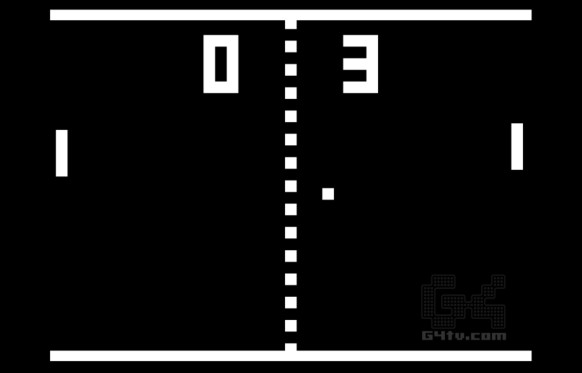
\includegraphics[width=0.45\linewidth]{Pong.jpg}
  \caption{Interfaz cl\'asica de Pong.}
  \label{fig:pong}
\end{figure}



\subsection{Interacci\'on}

En el modo continuo ser\'a frecuente la interacci\'on con los usuario v\'ia teclado o rat\'on. 

\subsubsection{Teclado}

Las acciones de teclado puede utilizarse como evento en s\'i o para recoger los detalles de la tecla pulsada. Por ejemplo la
variable booleana \textit{keyPressed} se activa si una tecla es presionada, en cualquier otro caso es falsa. Adem\'as, dicha variable estar\'a 
activa mientras mantengamos la tecla permanezca.

El siguiente c\'odigo hace uso de dicha variable para desplazar una l\'inea. 

\begin{lstlisting}[frame=single,caption={Ejemplo b\'asico},label=code:processing-primermmov]
int x = 20;
void setup() {
  size(100, 100);
  smooth();
  strokeWeight(4);
}
void draw() {
  background(204);
  if (keyPressed == true) 
  { 
    x++;   // incrementamos x
  }
  line(x, 20, x-60, 80);
}
\end{lstlisting}

Intenta modificarlo para dibujar dos l\'ineas diagonales que se desplazan.




Tambi\'en es posible recuperar la tecla pulsada. La variable \textit{key} es de tipo char y almacena el valor de la tecla que ha sido
presionada recientemente.

Este ejemplo muestra la tecla pulsada.

\begin{lstlisting}[frame=single,caption={Muestra la tecla},label=code:processing-tecla]
void setup() {
  size(100, 100);
}

void draw() {
  background(0);
  text(key, 28, 75);
}
\end{lstlisting}

Por supuesto, cada letra tiene un valor num\'erico en la Tabla ASCII, que tambi\'en podemoos mostrar

\begin{lstlisting}[frame=single,caption={El c\'odigo ASCII de la tecla},label=code:processing-teclaascii]
void setup() {
  size(100, 100);
}

void draw() {
  background(200);
  if (keyPressed == true) 
  {
    int x = key;
    text(key+" ASCII "+x, 20, 20 );
  }
}
\end{lstlisting}

Una particularidad interesante es poder identificar las teclas especiales como por ejemplo: flechas, \textit{Shift}, \textit{Backspace}, 
tabulador y otras m\'as. 
Para ello, lo primero que debemos hacer es comprobar si se trata de una de estas teclas comprobando el valor de la variable $key == CODED$.
El siguiente c\'odigo utilizando las teclas de las flechas cambie la posici\'on de una figura dentro del lienzo. 


\begin{lstlisting}[frame=single,caption={Ejemplo b\'asico},label=code:processing-teclaespecial]
color y = 35;
void setup() {
  size(100, 100);
}
void draw() {
  background(204);
  line(10, 50, 90, 50);
  if (key == CODED) 
  {
    if (keyCode == UP) 
    {
      y = 20;
    } 
    else 
      if (keyCode == DOWN) 
      {
        y = 50;
      }
  } 
  else 
  {
    y = 35;
  }
  rect(25, y, 50, 30);
}
\end{lstlisting}

Existe la posibilidad de detectar eventos individualizados, es decir el pulsado de una tecla en concreto. 
El siguiente ejemplo realiza una acci\'on al pulsar la tecla t.

\begin{lstlisting}[frame=single,caption={Ejemplo b\'asico evento de teclado},label=code:processing-eventos]
boolean drawT = false;

void setup() {
  size(100, 100);
  noStroke();
}

void draw() {
  background(204);
  if (drawT == true) 
  {
    rect(20, 20, 60, 20);
    rect(39, 40, 22, 45);
  }
}  
void keyPressed() 
{
  if ((key == 'T') || (key == 't')) 
  {
    drawT = true;
  }
}

void keyReleased() {
  drawT = false;
}
\end{lstlisting}

\textbf{Crea un ejemplo que modifique el color del fondo pulsando cada vocal.}


\subsubsection{Rat\'on}

En ejemplos previos hemos visto que es posible acceder a las coordenadas del rat\'on, simplemente 
haciendo uso de las variables
adecuadas desde el m\'etodo \textit{draw()} como en el c\'odigo siguiente.


\begin{lstlisting}[frame=single,caption={Ejemplo de uso de las coordenadas del rat\'on},label=code:processing-mouse]
void setup() {
  size(200, 200);
  rectMode(CENTER);
  noStroke();
  fill(0, 102, 153, 204);
}

void draw() {
  background(255);
  rect(width-mouseX, height-mouseY, 50, 50);
  rect(mouseX, mouseY, 50, 50);
}
\end{lstlisting}

Tambi\'en es posible usar el evento, es decir, la funci\'on que asociada con el mismo, 
como en este ejemplo que cambia el color del fondo.

\begin{lstlisting}[frame=single,caption={Ejemplo de cambio del tono de fondo},label=code:processing-gray]
 float gray = 0;
void setup() {
  size(100, 100);
}
void draw() {
  background(gray);
}
void mousePressed() {
  gray += 20;
}

\end{lstlisting}

El siguiente ejemplo usa el evento de pulsado para pasar del modo b\'asico al continuo.

\begin{lstlisting}[frame=single,caption={Paso a modo continuo},label=code:processing-continuo]
void setup()
{
  size(200, 200); 
  stroke(255); 	
  noLoop();
}

float y = 100;
void draw()
{
  background(0);   
  line(0, y, width, y);
  line(0, y+1, width, y+1);  
  y = y - 1;
  if (y < 0) {	y = height;  }
}

void mousePressed()
{
  loop();
}
\end{lstlisting}


Como puedse ver \textit{mousePressed()} es una funci\'on enlazada a la acci\'on de 
pulsar un bot\'on del rat\'on. Siendo posible controlar tambi\'en cuando
se suelta, se mueve, o si se arrastra el rat\'o con un bot\'on pulsado.

\begin{lstlisting}[frame=single,caption={Ejemplo evento de arrastre},label=code:processing-arrastre]
int dragX, dragY, moveX, moveY;
void setup() {
  size(100, 100);
  smooth();
  noStroke();
}  
void draw() {
  background(204);
  fill(0);
  ellipse(dragX, dragY, 33, 33); // C\'irculo negro
  fill(153);
  ellipse(moveX, moveY, 33, 33); // C\'irculo gris
}
void mouseMoved() { // Mueve el gris
  moveX = mouseX;
  moveY = mouseY;
}
void mouseDragged() { // Mueve el negro
  dragX = mouseX;
  dragY = mouseY;
}
 
\end{lstlisting}
 
\textbf{Mueve un objeto reflejando el movimiento del rat\'on.}

\subsection{Creando un Paint}

Como ya sabemos, las coordenadas de rat\'on se almacenan en las variables \textit{mouseX} y \textit{mouseY}.

\begin{lstlisting}[frame=single,caption={Coordenadas del rat\'on},label=code:processing-coormouse]
void setup() {
  size(640, 360); 
  noStroke();  
}

void draw() { 
  background(51); 
  ellipse(mouseX, mouseY, 66, 66);
}
\end{lstlisting}

Ambas son variables conteniendo las posiciones actuales del rat\'on, las previas est\'an disponibles
en \textit{pmouseX} y \textit{pmouseY}. Podemos utilizar las coordenadas el rat\'on para pintar
a mano alzada.

\begin{lstlisting}[frame=single,caption={Pintado con el "`pincel"'},label=code:processing-pincel]
void setup(){
  size(400,400);
  
  background(128);
}

void draw(){  
  point(mouseX,mouseY);
}
\end{lstlisting}

Es posible restringir el pintado a s\'olo cuando se pulse un bot\'on del rat\'on, empleando una estructura condicional.

\begin{lstlisting}[frame=single,caption={Pintado cuando se pulsa},label=code:processing-pintaalpulsar]
void setup(){
  size(400,400);
  
  background(128);
}

void draw(){  
  
  if (mousePressed == true) {
      point(mouseX,mouseY);
  }
}
\end{lstlisting}

Utilizando el teclado, en concreto las teclas del cursor arriba y abajo, para cambiar grosor del pincel (y pintamos c\'irculo), 
y cualquier otra tecla para alterar el color. Se identifica primero si se ha pulsado una tecla, y luego la tecla  en concreto pulsada.

\begin{lstlisting}[frame=single,caption={Grosor y color del pincel con las teclas},label=code:processing-grosordemipincel]
int grosor=1;
int R=0,G=0,B=0;

void setup(){
  size(400,400);  
  background(128);
}

void draw(){  
  
  if (mousePressed == true) {
      point(mouseX,mouseY);
  }
  
  if (keyPressed == true) {
    if (keyCode == UP) {
      grosor = grosor+1;
      strokeWeight(grosor);
    } 
    else 
    {
      if (keyCode == DOWN) {
        if (grosor>1){
        grosor = grosor-1;
        strokeWeight(grosor);
        }
      } 
      else
      {
        R=(int)random(255);
        G=(int)random(255);
        B=(int)random(255);
      }
    }    
  }
  
  //Muestra del pincel
  noStroke();
  fill(128);
  rect(4,4,grosor+2,grosor+2);
  fill(R,G,B);
  ellipse(5+grosor/2,5+grosor/2,grosor,grosor);
  
  stroke(R,G,B);
}
\end{lstlisting}


Que el radio del pincel dependa del valor de \textit{x} o \textit{y}.

\begin{lstlisting}[frame=single,caption={Radio del pincel dependiente de rat\'on},label=code:processing-radiovariable]
void setup() {
  size(640, 360); 
  noStroke();
  rectMode(CENTER);
}

void draw() {
  background(51); 
  fill(255, 204);
  rect(mouseX, height/2, mouseY/2+10, mouseY/2+10);
  fill(255, 204);
  int inversaX = width-mouseX;
  int inversaY = height-mouseY;
  rect(inversaX, height/2, (inversaY/2)+10, (inversaY/2)+10);
}
\end{lstlisting}

% Eventos de rat\'on.
% 
% \begin{lstlisting}[frame=single,caption={Eventos de rat\'on},label=code:processing-eventosraton]
% void setup() {
%   size(640, 360);
%   noSmooth();
%   fill(126);
%   background(102);
% }
% 
% void draw() {
%   if (mousePressed) {
%     stroke(255);
%   } else {
%     stroke(0);
%   }
%   line(mouseX-66, mouseY, mouseX+66, mouseY);
%   line(mouseX, mouseY-66, mouseX, mouseY+66); 
% }
% \end{lstlisting}

Sugerir ejemplos dentro de
\textit{Archivo $\rightarrow$ Ejemplos},
seleccionando por ejemplo \textit{Topics $\rightarrow$ Motion $\rightarrow$ Bounce}, 
\textit{Basics $\rightarrow$ Input $\rightarrow$ Storinginput}, etc.

\section{Avanzado}

Las contribuciones o bibliotecas se pueden a\~nadir a trav\'es de
\textit{Herramientas $\rightarrow$ A\~nadir herramientas $\rightarrow$ Libraries} 
Por ejemplo a\~nadir \textit{Video} y \textit{Sound} para los ejemplos de dichas caracter\'isticas.


\begin{lstlisting}[frame=single,caption={Captura de c\'amara},label=code:processing-captura]
import processing.video.*;

Capture video;

void setup(){
  size(320,240);
  
  video = new Capture(this,320,240);
  
   // Lanza la captura
  video.start();  
  
  background(0);
}

void draw(){
  if (video.available()){
    video.read();
  }
  image(video,0,0);
}
\end{lstlisting}

\begin{lstlisting}[frame=single,caption={Captura de c\'amara mostrando la mitad superior umbralizada},label=code:processing-captura-modifica]
import processing.video.*;

Capture video;

void setup(){
  size(320,240);
  
  video = new Capture(this,320,240);
  
   // Lanza la captura
  video.start();  
  
  background(0);
}

void draw(){
  if ( video.available())
  { 
    video.read() ; 
    
    //Tama\~no de la imagen
    int dimension = video.width * video.height;
    
    //Carga p\'ixeles
    video.loadPixels();
    //Umbraliza la parte superior de la imagen
    for (int i=1;i<dimension/2;i++)
    {
        float  suma=red(video.pixels[i])+green(video.pixels[i])+red(video.pixels[i]);
        
        //umbraliza al valor intermedio
        if (suma<255*1.5)
        {
          video.pixels[i]=color(0, 0, 0);
        }        
        else
        {
          video.pixels[i]=color(255, 255, 255);
        }
    }
    //Actualiza p\'ixeles
    video.updatePixels();
  } 
image( video ,0 ,0) ; 
}
\end{lstlisting}


Reproduciendo un sonido, puedes encontrar wavs \href{http://freewavesamples.com/}{aqu\'i}.

\begin{lstlisting}[frame=single,caption={Reproduciendo sonido},label=code:processing-sonido]
import processing.sound.*;

int pos=0;
int mov=5;

SoundFile  sonido;

void setup(){
  size(400,400);
  
  sonido = new SoundFile(this,"E:/Intro Programacion con Processing Experto/Bass-Drum-1.wav");
}   
   
void draw(){
  background(128);
  ellipse(pos,30,30,30);
  
  pos=pos+mov;
  
  if (pos>=400 || pos<=0){
    mov=-mov;
    sonido.play ( ) ; 
  }
}
\end{lstlisting}

Solventar la latencia del sonido con un hilo y el m\'etodo \textit{thread}.

\begin{lstlisting}[frame=single,caption={Latencia del sonido},label=code:processing-sonidolatencia]
import processing.sound.*;

int pos=0;
int mov=5;

SoundFile  sonido;

void setup(){
  size(400,400);
  
  sonido = new SoundFile(this,"E:/Intro Programacion con Processing Experto/Bass-Drum-1.wav");
}   
   
void draw(){
  background(128);
  ellipse(pos,30,30,30);
  
  pos=pos+mov;
  
  if (pos>=400 || pos<=0){
    mov=-mov;
    thread ("Suena");  
  }
}

void Suena( ) {  
  sonido.play ( ) ;
}
\end{lstlisting}






%\subsection{Pesta\~nas, varios archivos y clases}
%
%Puede ser un inconveniente para escribir un programa largo en un s\'olo archivo. Cuando los programas tienen muchas l\'ineas de c\'odigo, 
%romperlo en unidades modulares ayuda a gestionar las diferentes partes. Processing gestiona los archivos con el Sketchbook  y 
%cada dibujo puede tener varios archivos que se manejan con pesta\~nas. El bot\'on de la flecha en la esquina superior derecha del 
%entorno de trabajo nos permite generar nuevos ficheros. Haga clic en este bot\'on para mostrar las opciones para crear una nueva 
%pesta\~na, cambiar el nombre de la pesta\~na actual, y eliminar la pesta\~na actual. Si un proyecto tiene m\'as de una pesta\~na, sino que 
%tambi\'en puede ser escondido y revelado. Ocultar una pesta\~na quita temporalmente que el c\'odigo del sketch (no ser\'a compilado con el 
%programa cuando se presiona Ejecutar).
%
%Las pesta\~nas est\'an destinadas a usuarios m\'as avanzados, y por esta raz\'on, el men\'u que controla las pesta\~nas est\'a intencionalmente 
%puesto en un lugar menos prominente.



 
 \section{Tipos de datos}

Processing est\'a basado en Java, por lo que puedes utilizar cualquier caracter\'istia de dicho lenguaje en Processing. 
Recordamos algunos aspectos b\'asicos.

En Processing las variables se deben declarar expl\'icitamente y asignar las variables antes de llamar o de realizar una operaci\'on
sobre ellas. Para declarar una variable utilice una sintaxis similar a los ejemplos a continuaci\'on:

\begin{lstlisting}[frame=single,caption={Ejemplos de tipos de variables},label=code:processing-tiposdedatos]
// Cadenas
String myName = "supermanoeuvre";
String mySentence = " was born in ";
String myBirthYear = "2006";  

// Concatenar
String NewSentence = myName + mySentence + myBirthYear;
System.out.println(NewSentence);
 
// Enteros 
int myInteger = 1;
int myNumber = 50000;
int myAge  	= -48;
 
// Reales
float myFloat = 9.5435;
float timeCount = 343.2;
 
// Booleanos // True o False
boolean mySwitch = true;
boolean mySwitch2 = false;
\end{lstlisting}

Ejemplos de accesos a vectores.

\begin{lstlisting}[frame=single,caption={Uso de vectores},label=code:processing-arrays]
%\begin{lstlisting}[style=C++]
// Lista de Cadenas
String [] myShoppingList = new String[3];
myShoppingList[0] = "bananas";
myShoppingList[1] = "coffee";
myShoppingList[2] = "tuxedo";
 
// Lista de enteros
int [] myNumbers = new int[4];
myNumbers[0] = 498;	
myNumbers[1] = 23; 	
myNumbers[2] = 467;	
myNumbers[3] = 324;	
 
// printamos un dato de la lista
println( myNumbers[2] );  

int a = myNumbers[0] + myNumbers[3];   
println( a );     
\end{lstlisting}


Processing incluye la clase \textit{ArrayList} de Java, que no requiere conocer su tama\~no desde el inicio. De esta forma se facilita a\~nadir objetos
a la lista, ya que el tama\~no de la lista aumenta o decrece de forma autom\'atica. 

\begin{lstlisting}[frame=single,caption={Uso del tipo ArrayList},label=code:processing-arraylist]
ArrayList lista = new ArrayList();
int i = 0;

while (i<4){
  lista.add(i+3);
  i=i+1;
}

println("\nLos datos son: \n");
Iterator iter = lista.iterator();
while(iter.hasNext()){
  println(iter.next());
}

ArrayList myVectorList ;
myVectorList = new ArrayList();
 
// Asignamos objectos
myVectorList.add( new PVector(51,25,84) );
myVectorList.add( new PVector(98,3,54) );
 
// o //
PVector myDirection = new PVector(98,3,54);
myVectorList.add( myDirection  );
 
// Bucle para acceder a objetos usando ArrayList.size() y ArrayList.get()
for(int i = 0; i < myVectorList.size(); i++){
PVector V = (PVector) myVectorList.get(i);  // ojo con el cast (PVector)
println(V);
}
 
\end{lstlisting}

\section{Applets}

Una vez finalizado el proceso de prueba de un boceto, es posible exportarlo generando un ejecutable. Para ello mediante la opci\'on
 \textit{File $\rightarrow$ Export Application}, habiendo escogido el modo Javascript en el botón de la parte superior derecha, se genera el correspondiente applet con su fichero html para su carga con un navegador. Puedes probar on cualquiera de los ejemplos.



\section{Utilidades gr\'aficas}

Processing incorpora funciones que hacen m\'as f\'acil el manejo de objetos gr\'aficos, como por ejemplo las transformaciones: traslaci\'on, rotaci\'on y escalado.
Recuerda sin embargo que estas utilidades no puedes emplearlas para obtener los objetivos de la pr\'actica, pero siempre podr\'as conocerlas
para elementos de la interfaz o un futuro.

Para ilustrar la traslaci\'on, en las im\'agenes mostramos un cuadrado antes y despu\'es de trasladarlo, como se ve en la figura~\ref{fig:Rect}.

\begin{figure}[hbt]  
\begin{minipage}[t]{1.0\linewidth}
    \centering
    \centering
    \begin{minipage}[c]{0.5\linewidth}
      \centering
      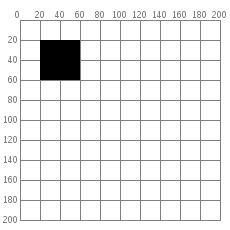
\includegraphics[width=0.9\linewidth]{processing-rect.png}\\
      %(a)
    \end{minipage}\hfill
     \begin{minipage}[c]{0.5\linewidth}
      \centering
      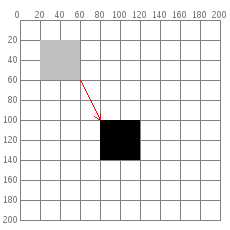
\includegraphics[width=0.9\linewidth]{processing-rectT.png}\\
      %(a)
    \end{minipage}\hfill 
   
    \vspace{0.18cm}
     \caption{Cuadrado antes y tras trasladar.
     \label{fig:Rect}}
  \end{minipage}
\end{figure}

Si desea mover el cuadrado $60$ unidades a la derecha y $80$ unidades hacia abajo, puedes cambiar las coordenadas mediante la suma a los puntos iniciales: $rect (20 + 60, 20 + 80, 40, 40)$ y el cuadrado aparecer\'a en un lugar diferente. %(Hemos puesto la flecha en la que para el efecto dram\'atico.)


La traslaci\'on puede realizarse desplazando el cuadrado un n\'umero determinado de coordenadas, pero tambi\'en obtenemos un efecto similar si movemos
el sistema de coordenadas. %Mover el sistema de coordenadas  se llama traslaci\'on.

 
\begin{figure}[ht]
  \centering
  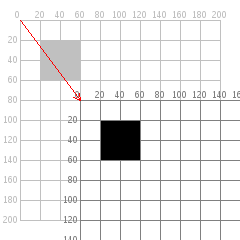
\includegraphics[scale=0.7]{processing-rectT2.png}
  \caption{Traslaci\'on del sistema de referencia}
  \label{fig:processing_rectT}
\end{figure}
 
 Lo importante a notar en el diagrama anterior es que, el rect\'angulo no se ha movido de su posici\'on, su esquina superior izquierda se encuentra todav\'ia en (20,20), por el contrario, el sistema de coordenadas se modifica. Incluimos el c\'odigo que realiza el movimiento del cuadrado de las dos formas.
 
  \begin{lstlisting}[frame=single,caption={Traslaci\'on del sistema de referencia},label=code:processing-traslacion]
 void setup()
{
  size(200, 200);
  background(255);
  noStroke();
  // Dibuja el primer objeto 
  fill(192);
  rect(20, 20, 40, 40);
  // Dibuja otro desplazado
  fill(255, 0, 0, 128);
  rect(20 + 60, 20 + 80, 40, 40);
  
  // Este nuevo objeto tiene las mismas coordenadas que el primero pero antes hemos movido el sistema de referencia
  fill(0, 0, 255, 128);
  pushMatrix(); //Salva el sistema de coordenadas actual
  translate(60, 80);
  rect(20, 20, 40, 40);
  popMatrix(); //vuelve al sistema de coordenadas original
}
\end{lstlisting}
 
 
 Modificar el sistema de coordenadas puede ser engorroso para un ejemplo tan sencillo como el cuadrado. Pero tomemos un ejemplo donde \textit{translate()} puede hacer la vida algo m\'as f\'acil. El siguiente c\'odigo dibuja una hilera de casas usando los dos esquemas. Se utiliza un bucle que llama a la funci\'on llamada \textit{house()}, que tiene la ubicaci\'on X e Y de la esquina superior izquierda de la casa como sus par\'ametros.
 
 
 \begin{lstlisting}[frame=single,caption={Dibujo de varias casas},label=code:processing-casa]
void setup()
{
  size(400, 400);
  background(255);
  for (int i = 10; i < 350; i = i + 50)
  {
    house(i, 20);
  }
}

void house(int x, int y)
{
  triangle(x + 15, y, x, y + 15, x + 30, y + 15);
  rect(x, y + 15, 30, 30);
  rect(x + 12, y + 30, 10, 15);
}

**************************************************

void setup()
{
  size(400, 400);
  background(255);
  for (int i = 10; i < 350; i = i + 50)
  {
		house(i, 20);
  }
}

void house(int x, int y)
{
  pushMatrix();
  translate(x, y);
  triangle(15, 0, 0, 15, 30, 15);
  rect(0, 15, 30, 30);
  rect(12, 30, 10, 15);
  popMatrix();
}
}
\end{lstlisting}



Tambi\'en se pueden aplicar otras transofrmaciones como la rotaci\'on con la funci\'on \textit{rotate()}. Esta funci\'on tiene un argumento, que es el n\'umero de radianes que desea girar. En Processing, todas las funciones que tienen que ver con medir \'angulos de rotaci\'on en radianes en lugar de grados. Cuando
se habla de \'angulos en grados, se dice que un c\'irculo completo son $360^o$. Cuando se habla de los \'angulos en radianes, se dice que un c\'irculo
completo tiene $2\pi$ radianes. Aqu\'i hay un diagrama de c\'omo Processing mide los \'angulos en grados (negro) y radianes (rojo).
 
\begin{figure}[ht]
  \centering
  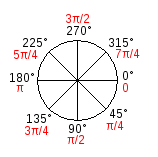
\includegraphics[scale=0.5]{processing_angulos.png}
  \caption{\'Angulos de rotaci\'on en grados y radianes}
  \label{fig:processing_angulos}
\end{figure} 

Como la mayor\'ia de la gente piensa en grados, Processing tiene una funci\'on integrada \textit{radians()} que toma un n\'umero de grados como 
su argumento y lo convierte para ti. Tambi\'en tiene la funci\'on de \textit{degrees()} que convierte radianes a grados. 
Teniendo en cuenta estos antecedentes, vamos a intentar girar un cuadrado de $45$ grados en sentido horario.

\begin{lstlisting}[frame=single,caption={Rotaci\'on},label=code:processing-ratacion]
void setup()
{
  size(200, 200);
  background(255);
  smooth();
  fill(192);
  noStroke();
  rect(40, 40, 40, 40);
 
  pushMatrix();
  rotate(radians(45));
  fill(0);
  rect(40, 40, 40, 40);
  popMatrix();
}
\end{lstlisting}


\begin{figure}[ht]
  \centering
  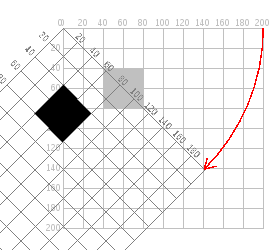
\includegraphics[scale=0.8]{processing-rectR.png}
  \caption{Rotaci\'on del cuadrado}
  \label{fig:processing_rectR}
\end{figure} 


La forma correcta de hacer girar el cuadrado es:

\begin{enumerate}
	\item Trasladar el origen del sistema de coordenadas de (0, 0) a donde desea que la parte superior izquierda que desee del cuadrado.
	\item Gire la red de $\pi/4$ radianes ($45^o$)
	\item Dibuja el cuadrado en el origen.
\end{enumerate}
 

\begin{lstlisting}[frame=single,caption={Transformaci\'on},label=code:processing-transforma]
void setup()
{
  size(200, 200);
  background(255);
  smooth();
  fill(192);
  noStroke();
  rect(40, 40, 40, 40);
  
  pushMatrix();
  // mueve el origen al punto pivote
  translate(40, 40); 
  
  // rota sobre ese punto pivote
  rotate(radians(45));
  
  // y dibuja el cuadrado
  fill(0);
  rect(0, 0, 40, 40);
  popMatrix(); //luego reestablece el grid
}
\end{lstlisting}

Por \'ultimo el escalado como en el siguiente ejemplo modifica el aspecto del cuadrado.

\begin{lstlisting}[frame=single,caption={Escalado},label=code:processing-escalado]
void setup()
{
  size(200,200);
  background(255);
  
  stroke(128);
  rect(20, 20, 40, 40);
  
  stroke(0);
  pushMatrix();
  scale(2.0);
  rect(20, 20, 40, 40);
  popMatrix();
}
\end{lstlisting}

En primer lugar, parece que el cuadrado se ha movido, pero nada de eso. Su esquina superior izquierda se encuentra todav\'ia en la 
posici\'on (20, 20). Tambi\'en se puede ver que las l\'ineas son m\'as gruesas. Eso no es una ilusi\'on \'optica, las l\'ineas son
en realidad dos veces m\'as gruesas, porque el sistema de coordenadas se ha reducido al doble de su tama\~no.

Al hacer m\'ultiples transformaciones, el orden es importante. Una rotaci\'on seguida de una traslaci\'on seguido de una escala que no 
dar\'a los mismos resultados que una trasladar seguido de una rotaci\'on por una escala. 

\begin{lstlisting}[frame=single,caption={Encadenando transformaciones},label=code:processing-transformaciones]
void setup()
{
  size(200, 200);
  background(255);
  smooth();
  line(0, 0, 200, 0); // dibuja bordes de la imagen
  line(0, 0, 0, 200);
  
  pushMatrix();
  fill(255, 0, 0); // cuadrado rojo
  rotate(radians(30));
  translate(70, 70);
  scale(2.0);
  rect(0, 0, 20, 20);
  popMatrix();

  pushMatrix();
  fill(255); // cuadrado blanco
  translate(70, 70);
  rotate(radians(30));
  scale(2.0);
  rect(0, 0, 20, 20);
  popMatrix();
}
\end{lstlisting}

Cada vez que haces una rotaci\'on, traslaci\'on, o escalado, la informaci\'on necesaria para realizar la transformaci\'on se va acumulando en una matriz. Esta matriz contiene toda la informaci\'on necesaria para hacer cualquier serie de transformaciones. Y esa es la raz\'on por la que se usan las funciones \textit{pushMatrix()} y \textit{popMatrix()}.

Las funciones nos permiten manejar una pila de sistemas de referencia, \textit{pushMatrix()} pone el estado actual del sistema de 
coordenadas en la parte superior de un \'area de memoria, y \textit{popMatrix()} que extrae el estado de nuevo hacia fuera. 
El ejemplo anterior utiliza \textit{pushMatrix()} y \textit{popMatrix()} para asegurarse de que el sistema de coordenadas estaba \textit{limpio} antes de cada parte del dibujo. En todos los otros ejemplos, las llamadas a esas dos funciones no eran realmente necesarias, pero no hace da\~no salvar y restaurar el estado del grid.

En Processing, el sistema de coordenadas se restaura a su estado original (de origen en la parte superior izquierda de la ventana, sin rotaci\'on ni escalado) cada vez que la funci\'on \textit{draw()} se ejecuta.


Para trabajar en tres dimensiones basta con pasar tres argumentos a las funciones de transformaci\'on. Para las rotaciones haremos uso de las funciones \textit{rotateX()}, \textit{rotateY()}, o \textit{rotateZ()}.




\section{Referencias y fuentes}

Algunas fuentes de informaci\'on:

\begin{itemize}
  \item \href{http://processing.org/}{Processing} y \href{http://processing.org/reference/}{Processing reference}
	%\item \href{http://www.openframeworks.cc/documentation/}{Documentaci\'on oficial de openFrameworks}
	%\item \href{http://www.openframeworks.cc/tutorials/}{Tutoriales de openFrameworks}
	%\item \href{http://forum.openframeworks.cc/}{Foro de openFrameworks}
	\item \href{https://processing.org/exhibition/}{Processing exhibition archives}
  \item \href{http://shop.oreilly.com/product/0636920021735.do}{Programming Interactivity}, Joshua Noble, 2nd edition, O'Reilly, 2012. Libro que cubre tanto Processing como otras entornos openFrameworks como Arduino. \href{http://proquest.safaribooksonline.com/book/programming/graphics/9781449321482}{Enlace desde la red de la universidad.} 
  \item \href{http://processing.lyndondaniels.com/}{An Introduction To Programming With Processing}
\item \href{http://funprogramming.org/}{Fun programming}
\item \href{http://openprocessing.org/}{openProcessing share your sketches}
\item \href{http://www.openprocessing.org/collection/25}{OpenProcessing games}
\item \href{http://www.creativeapplications.net/}{Creative Applications Net}
\end{itemize}

 
\end{document}
